\documentclass{standalone}
\usepackage{tikz}
\usepackage{amsmath}
\usetikzlibrary{patterns}

\begin{document}
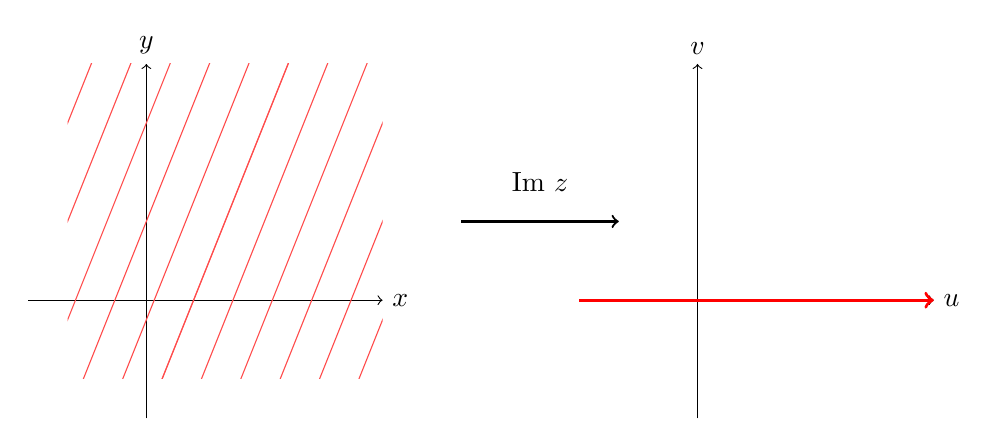
\begin{tikzpicture}[scale=1]

  % First coordinate system (z-plane)
  \begin{scope}[shift={(0,0)}]
    \draw[->] (-1.5,0) -- (3,0) node[right] {$x$};
    \draw[->] (0,-1.5) -- (0,3) node[above] {$y$};
    % \node[above] at (1.5, 2.5) {Im $z$};

    % Shaded region (using patterns library)
    \begin{scope}
      \clip (-1,-1) rectangle (3,3); % Clip to avoid drawing outside the axes
% \draw[pattern=north east lines, pattern color=red!70] (0,0) -- (2,2) -- (0,2) -- cycle;
      \foreach \i in {-3.5,,-3,-2.5,-2,...,3.5}{
          \draw[red!70] (\i-1, {-4}) -- ({\i+2}, 3.5);
      }
    \end{scope}

        % \draw[fill=red!70] (-0.5,-0.5) circle (1pt);
        % \draw[fill=red!70] (0.5,0.5) circle (1pt);
        % \draw[fill=red!70] (1,1) circle (1pt);
  \end{scope}

  % Arrow between coordinate systems
  \draw[->, thick] (4,1) -- (6,1);
  \node[above] at (5, 1.25) {Im $z$};


  % Second coordinate system (w-plane)
  \begin{scope}[shift={(7,0)}]
    \draw[->] (-1.5,0) -- (3,0) node[right] {$u$};
    \draw[->,] (0,-1.5) -- (0,3) node[above] {$v$};

    % Line segment in the w-plane
    \draw[->, red, very thick] (-1.5,0) -- (3,0);
  \end{scope}

\end{tikzpicture}
\end{document}